\section{PDEs by Separation of Variables}

This method works for linear PDEs whose variables are separable, i.e., PDEs for which some solutions can be written as products of functions of the two independent variables:
\[
u(x,t) = f(x)g(t)
\]

\subsection{The Heat Equation}

To give a bit of background about the heat equation:
\begin{itemize}
	\item The heat equation can be used to describe the evolution of temperature in a one-dimensional object. If we imagine a thin rod, its temperature will depend only on the position $x$ of the particles between $0$ and $L$, and the time $t$. \\
	The heat equation describes how this temperature changes as a function of time. As time evolves, the temperature differences across the rod decrease because the conduction of heat across the rod conducts energy from areas of high temperature to low temperature. In this case, we will take the boundary conditions of $u$ to be 0 when $x=0$ and $x=L$; this corresponds to setting the temperature to 0 at these ends.
	
	\item Similarly, the heat equation can also be applied to Brownian motion or random walks. It describes the probability density function of particles that move randomly according to Brownian movements. Brownian motion is the limit of a random walk where walkers take many steps in very short intervals of time. The boundary conditions in this case are the points where we get rid of particles that touch any end of the walk. So at $x=0$ and $x=L$ again.
\end{itemize}

The heat equation is given by 
\begin{equation}\label{eq5.1}
	\p_t u = \alpha^2 \p_{xx} u,
\end{equation} 
where $\alpha > 0$. $\alpha^2$ is called the thermal diffusivity.

The boundary conditions are given by
\[
u(0,t) = u(L,t) = 0,
\]
and the initial conditions are given by
\[
u(x,0) = f(x).
\]
This corresponds to modelling the temperature in a rod given an initial temperature distribution $f(x)$ and where we set the temperature to zero at both ends of the rod, as shown in \Cref{fig:heateqnrod}.

\begin{figure}[!ht]
	\centering
	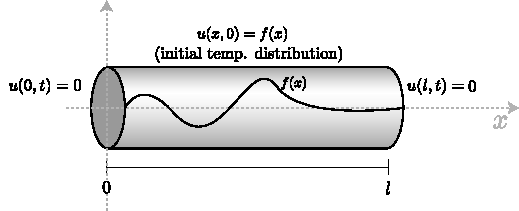
\includegraphics[width=0.7\textwidth]{HeatEqnRod.pdf}
	\caption{Modelling the temperature in a rod using the heat equation with homogeneous boundary conditions (source: \href{https://commons.wikimedia.org/wiki/File:Temp_Rod_homobc.svg}{Wikimedia}).}
	\label{fig:heateqnrod}
\end{figure}

We can solve the heat equation by separation of variables as follows: we look for solutions $u(x,t)$ as a product of two functions which have independent variables. So, try:
\begin{equation}\label{eq5.2}
	u(x,t) = X(x) T(t).
\end{equation}
Substituting \Cref{eq5.2} into \Cref{eq5.1}:
\begin{align*}
	XT' &= \alpha^2 X''T \\
	\implies \frac{1}{\alpha^2} \frac{T'}{T} &= \frac{X''}{X}.
\end{align*}
Now we have a function of only $x$ on the RHS and only $t$ on the LHS. This is possible only if $\frac{1}{\alpha^2} \frac{T'}{T} = \frac{X''}{X} = \lambda$ where $\lambda$ is a constant, called the separation constant. So, now we have two ODEs:
\[
X'' = \lambda X \quad\text{and}\quad T' = \lambda \alpha^2 T.
\]
To find solutions for $X(x)$, we have boundary conditions $X(0) = X(L) = 0$, so we now want non-trivial solutions to $X(x)$. What we have now is the eigenvalue problem from \Cref{eg:eigenvalprob} where $\lambda$ is the eigenvalue.

We consider three cases:
\begin{itemize}
	\item Case 1: $\lambda = \mu^2 > 0$.\\
	The ODE is given by: $X'' - \mu^2X = 0$.\\
	In this case, the solution is given by:
	\[
	X(x) = A \cosh{\mu x} + B \sinh{\mu x}.
	\]
	Using the boundary values:
	\begin{align*}
		X(0) &= A = 0 \\
		X(L) &= B \sinh{\mu L} = 0 \implies B=0.
	\end{align*}
	So, there are only trivial solutions in this case.
	
	\item Case 2: $\lambda = 0$.\\
	The ODE is given by: $X''= 0$.\\
	In this case, the solution is given by:
	\[
	X(x) = Ax + B.
	\]
	Using the boundary values:
	\begin{align*}
		X(0) &= B = 0 \\
		X(L) &= AL = 0 \implies A = 0.
	\end{align*}
	So, there are only trivial solutions in this case.
	
	\item Case 3: $\lambda = -\mu^2 < 0$.\\
	The ODE is given by: $X'' + \mu^2 X = 0$.\\
	In this case, the solution is given by:
	\[
	X(x) = A \cos{\mu x} + B \sin{\mu x}.
	\]
	Using the boundary values:
	\begin{align*}
		X(0) &= A = 0 \\
		X(L) &= B \sin{\mu L} = 0.
	\end{align*}
	In this case, however, $B \neq 0$ if $\mu L = n \pi$ where $n \in \Z$. So, we have non-trivial solutions $\lambda = -\mu^2$ where $\mu = \frac{n \pi}{L}$.
\end{itemize}
Thus, the eigenvalues are given by: $\lambda = -\frac{n^2\pi^2}{L^2}$, where $n = 1, 2, \dots$, and the eigenfunctions are given by: $X_n(x) = \sin\left(\frac{n\pi x}{L}\right)$.

To find solutions for $T(t)$:
\begin{align*}
	T' &= \alpha^2 \lambda T \\
	T_n' &= -\frac{\alpha^2 n^2 \pi^2}{L^2} T_n \\ 
	\implies T_n(t) &= e^{-\alpha^2 n^2 \pi^2 t/L^2}.
\end{align*}
Therefore we have a linear set of solutions of the form:
\[
u_n(x,t) = X_n(x)T_n(t) = \sin\left(\frac{n\pi x}{L}\right) e^{-\alpha^2 n^2 \pi^2 t/L^2}
\]
To get a general solution, we use superposition:
\begin{equation}\label{eq:heateqsol}
	u(x,t) = \sum_{n=1}^{\infty} c_n e^{-\alpha^2 n^2 \pi^2 t/L^2} \sin\left(\frac{n\pi x}{L}\right).
\end{equation}
In order to satisfy the initial condition, we require
\[
u(x,0) = \sum_{n=1}^{\infty} c_n \sin\left(\frac{n\pi x}{L}\right) = f(x),
\]
which we observe is nothing but the Fourier series for an odd function (or odd extension). Using the Euler-Fourier formulas from \Cref{sec:evenoddfourier}, we have that
\begin{equation}\label{eq:heatfourier}
	c_n = \frac{2}{L} \int_0^L f(x)\sin\left(\frac{n\pi x}{L}\right) dx.
\end{equation}

It is important to check that the infinite sum in \Cref{eq:heateqsol} converges. For $t=0$, if $f(x)$ and $f'(x)$ are piecewise continuous, then the Fourier convergence theorem (\Cref{thrm:fourierconv}) guarantees convergence at $t=0$. For $t>0$, the decreasing exponential dependence in $t$ suggests the series will converge. This will be addressed in \Cref{sec:slmain} on Sturm-Liouville theory.

\begin{eg}\label{eg:heateqn1}
	We solve the heat equation with boundary conditions given by: $u(0,t) = u(1,t) = 0$, and initial conditions $u(x,0) = f(x)$, where $f$ is the tent function given by
	\[
	f(x) = \begin{cases} 2x & \text{if } x \leq \frac12 \\ 2(1-x) & \text{if } x>\frac12 \end{cases}.
	\]
	Since $L=1$,\footnote{This derivation is done in more detail in \Cref{eg:laplacerect}.}
	\begin{align*}
		c_n &= 2 \int_0^1 f(x) \sin(n\pi x) \,dx \\
		&= 2 \int_0^{1/2} x \sin(n\pi x) \,dx + 2 \int_{1/2}^1 (1-x) \sin(n\pi x) \,dx \\
		&= \frac{4}{(n \pi)^2} \sin \left(\frac{n \pi}{2}\right) \\
		&= \begin{cases}0 & \text{if } n = 2k \\ \dfrac{4}{((2k+1)\pi)^2} (-1)^k & \text{if } n = 2k+1\end{cases}.
	\end{align*}
	Thus the solution is given by, 
	\[
	u(x,t) = \sum_{k=0}^{\infty} \frac{8}{((2k+1)\pi)^2} (-1)^k e^{-\alpha^2 n^2 \pi^2 t} \sin\left((2k+1)\pi x\right).
	\]
	This solution is shown in \Cref{fig:heateqneg1} for a few select values of $t$.
\end{eg}

\begin{figure}[!ht]
	\centering
	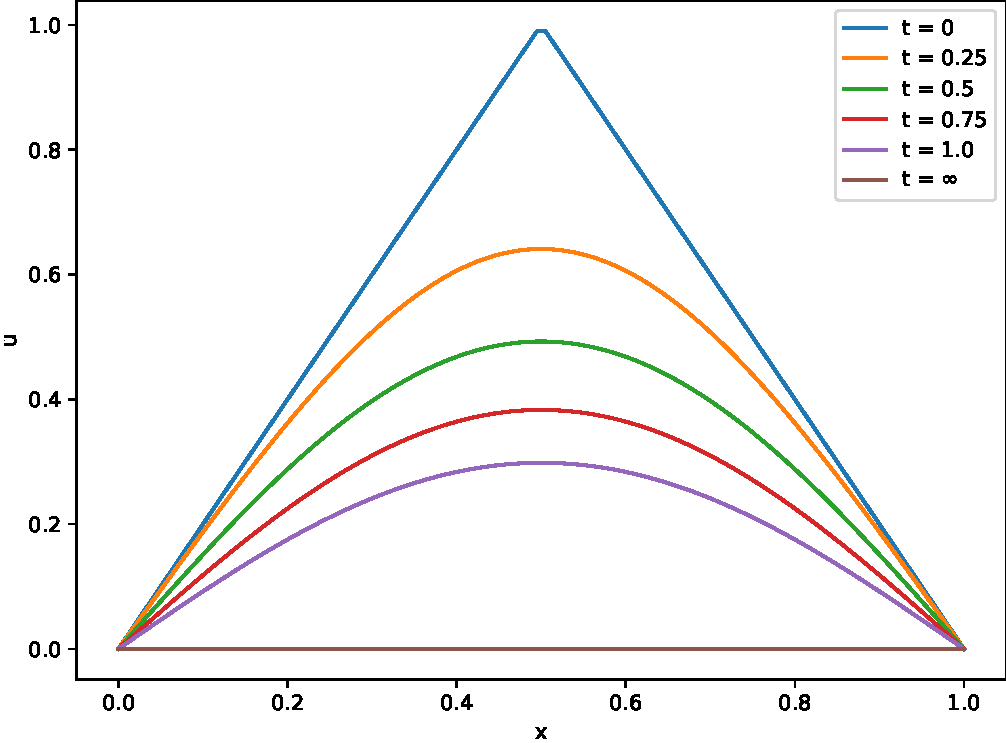
\includegraphics[width=0.7\textwidth]{HeatEqn1.pdf}
	\caption{Solution of the heat equation given the initial conditions in \Cref{eg:heateqn1}.}
	\label{fig:heateqneg1}
\end{figure}

\subsubsection{Non-homogenous Boundary Conditions}

We now wish to solve the heat equation 
\[
\p_t u = \alpha^2 \p_{xx} u
\]
with non-homogeneous (i.e. non-zero) boundary conditions:
\[
u(0,t) = a, \quad u(L,t) = b
\]
and initial condition
\[
u(x,0) = f(x).
\]

In the physical interpretation, this corresponds to keeping the ends of the rod at some fixed, finite temperature.

Let
\begin{equation}
	u(x,t) = v(x) + w(x,t),
\end{equation}
where $v(x)$ is a steady solution of the heat equation, meaning that it satisfies
\[
\p_{xx} v(x) = \frac{d^2}{dx^2} v = 0,
\]
and $v(0) = a$ and $v(L) = b$.
Since $u$ satisfies the heat equation, so do $v$ and $w$ by linearity of $u$. So,
\begin{align*}
	& \p_t u = \cancelto{0}{\p_t v(x)} + \p_t w(x,t) = \alpha^2 \left( \cancelto{0}{\p_{xx} v(x)} + \p_{xx} w \right)\\
	\implies & \p_t w(x,t) = \alpha^2 \p_{xx} w \\
	\implies & u(0,t) = v(0) + w(0,t) = a \\
	\implies & w(0,t) = 0.
\end{align*}
Similarly, we find that $w(L,t) = 0$.

Solving for $v(x)$:
\[
v'' = 0, \qquad v(0) = a, v(L) = b
\]
The solution is given by:
\begin{align*}
	v(x) &= Ax + B \\
	v(0) & = B = a \\
	v(L) & = AL + a = b \\
	\implies A &= \frac{b-a}{L}.
\end{align*}
So, we have
\[
v(x) = \frac{b-a}{L}x + a.
\]

Solving for $w(x,t)$, we know that $w(x,t)$ satisfies the heat equation with homogenous boundary conditions so 
\[
w(x,t) = \sum_{n=1}^{\infty} c_n e^{-\alpha^2 n^2 \pi^2 t/L^2} \sin\left(\frac{n\pi x}{L}\right),
\]
and
\begin{equation}
	u(x,t) = \frac{b-a}{L}x + a + \sum_{n=1}^{\infty} c_n e^{-\alpha^2 n^2 \pi^2 t/L^2} \sin\left(\frac{n\pi x}{L}\right).
\end{equation}
We now use the initial conditions at $t=0$, 
\begin{align*}
	u(x,0) &= f(x) \\
	v(x) + w(x,0) &= f(x) \\
	\implies w(x,0) &= f(x) - v(x).
\end{align*}
From \Cref{eq:heatfourier}, we have that 
\begin{equation}
	c_n = \frac{2}{L} \int_{-L}^L \left( f(x) - \frac{b-a}{L}x - a \right) \sin{\left(\frac{n \pi x}{L} \right)} dx.
\end{equation}

\begin{eg}\label{eg:heateqn2}
	Consider the heat equation
	\[
	\p_t u = \alpha^2 \p_{xx} u,
	\]
	given $L=1$ and boundary and initial conditions:
	\begin{align*}
		u(0,t) = 0 \\
		u(L,t) = 1 \\
		u(x,0) = 0.
	\end{align*} 
	Here, $v(x) = x$ since $b=1$, $a=0$, and $L=1$, so
	\[
	c_n = 2 \int_{0}^1 (-x) \sin{\left(n \pi x \right)} \,dx = \frac{2(-1)^n}{n \pi}.
	\]
	So the solution is
	\[
	u(x,t) = x + \frac{2}{\pi} \sum_{n=1}^{\infty} \frac{(-1)^n}{n} e^{-\alpha^2 n^2 \pi^2 t}\sin{\left(n \pi x \right)}.
	\]
	This solution is shown in \Cref{fig:heateqneg2} for a few select values of $t$.
\end{eg}

\begin{figure}[!ht]
	\centering
	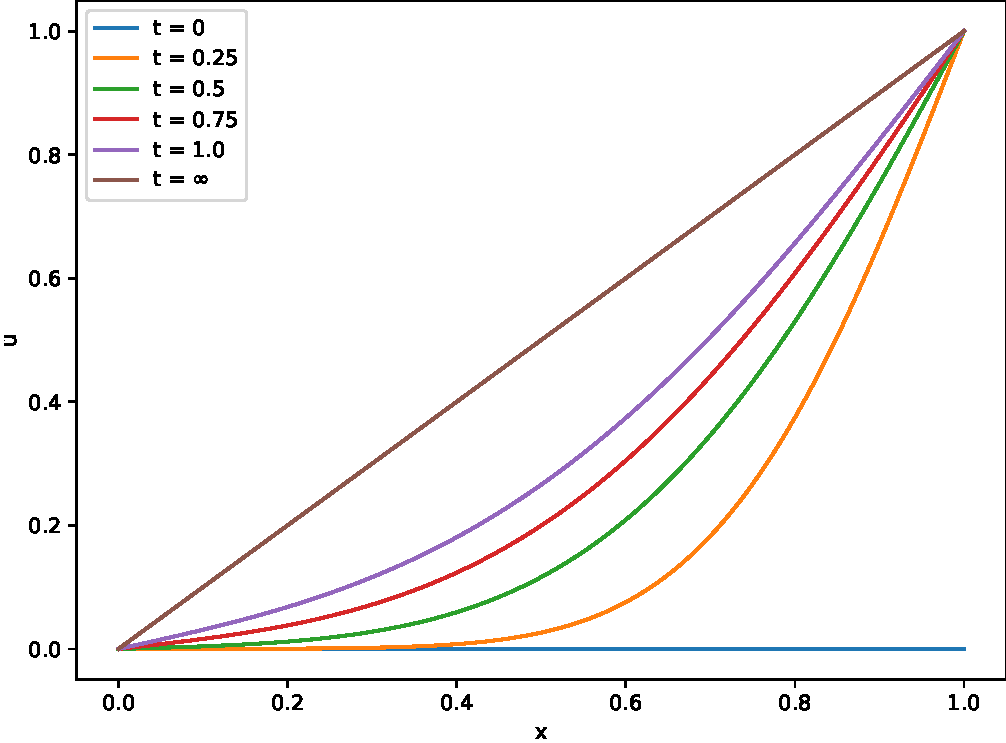
\includegraphics[width=0.7\textwidth]{HeatEqn2.pdf}
	\caption{Solution of the heat equation given the initial conditions in \Cref{eg:heateqn2}.}
	\label{fig:heateqneg2}
\end{figure}

\subsubsection{No-flux Boundary Conditions}

Finally, we wish to solve the heat equation
\[
\p_t u = \alpha^2 \p_{xx} u
\] 
with no-flux boundary conditions, i.e. where
\[
\p_x u(0,t) = \p_x u(L,t) = 0,
\]
and the typical initial conditions
\[
u(x,0) = f(x).
\]

This corresponds to both ends of the bar being insulated - the temperature does not vary with position at both ends of the bar.

Using the method of separation of variables:
\begin{align*}
	u(x,t) &= X(x) T(t) \\
	\frac{1}{\alpha^2} \frac{T'}{T} &= \frac{X''}{X} \\
	\implies X'' - \lambda X &= 0,
\end{align*}
where $X'(0) = X'(L) = 0$.

We then consider the separate cases of $\lambda$ as before:
\begin{itemize}
	\item Case 1: $\lambda = \mu^2 > 0$.\\
	The ODE is given by: $X(x)'' - \mu^2 X(x) = 0$.\\
	In this case, the solution is given by:
	\[
	X(x) = A \cosh{\mu x} + B \sinh{\mu x}.
	\]
	Using the boundary values:
	\begin{align*}
		X'(0) &= \mu B = 0 \implies B=0 \\
		X'(L) &= \mu A \cosh{\mu L} = 0 \implies A=0.
	\end{align*}
	So, there are only trivial solutions in this case.
	
	\item Case 2: $\lambda = 0$.\\
	The ODE is given by: $X''= 0$.\\
	In this case, the solution is given by:
	\[
	X(x) = Ax + B.
	\]
	Using the boundary values:
	\begin{align*}
		X'(0) &= A = 0 \\
		X'(L) &= AL = 0 \implies A = 0,
	\end{align*}
	which is true for all values of $B$. Therefore, the eigenvalue $\lambda_0 = 0$ has a corresponding eigenfunction given by $X(x) = 1$.
	
	\item Case 3: $\lambda = -\mu^2 < 0$.\\
	The ODE is given by: $X'' + \mu^2 X = 0$.\\
	In this case, the solution is given by:
	\[
	X(x) = A \cos{\mu x} + B \sin{\mu x}.
	\]
	Using the boundary values:
	\begin{align*}
		X'(0) &= \mu B = 0 \implies B = 0 \\
		X'(L) &= -\mu A \sin{\mu L} = 0 \implies \mu L = n \pi,
	\end{align*}
	where $n \in \Z \backslash \{0\} $. So, we have non-trivial solutions $\lambda = -\mu^2$ where $\mu = \frac{n \pi}{L}$.
\end{itemize}
Thus, the eigenvalues are given by: $\lambda_n = -\frac{n^2\pi^2}{L^2}$, and the eigenfunctions are given by: $X_n(x) = \cos{\left(\frac{n \pi x}{L} \right)}$.

Recall
\begin{align*}
	T' &= \lambda \alpha^2 T \\
	T_0(t) &= 1 \\
	T_n(t) &= e^{-\alpha^2 n^2 \pi^2 t/L^2}.
\end{align*}
So we have sets of solutions given by:
\[
u_n(x,t) = X_n(x) T_n(t) = \cos{\left(\frac{n \pi x}{L} \right)} e^{-\alpha^2 n^2 \pi^2 t/L^2}.
\]
By applying superposition, we can find the general solution to be:
\begin{equation}
	u(x,t) = \frac{c_0}{2} + \sum_{n=1}^{\infty} c_n e^{-\alpha^2 n^2 \pi^2 t/L^2} \cos{\left(\frac{n \pi x}{L} \right)}.
\end{equation}
Now considering the initial conditions:
\begin{align}
	u(x,0) & = f(x) \nonumber \\
	f(x) & = \frac{c_0}{2} + \sum_{n=1}^{\infty} c_n \cos{\left(\frac{n \pi x}{L} \right)} \nonumber \\
	\implies c_n & = \frac{2}{L} \int_0^L f(x) \cos{\left(\frac{n \pi x}{L} \right)} dx,
\end{align}
since this is nothing but the Fourier series for an even function.

\subsection{The Wave Equation}\label{sec:waveeqn}

We now solve another important partial differential equation: the wave equation,
\begin{equation}
	\p_{tt}u = a^2 \p_{xx}u, \quad a>0,
\end{equation}
where $a$ represents the wave speed.

In practice, this equation can be used to model a string under tension, or shallow water waves.

We will solve the equation with the following boundary conditions,
\[
u(0,t) = u(L,t) = 0,
\]
and the initial conditions
\[
u(x,0) = f(x), \quad \p_t u(x,0) = g(x).
\]
These conditions correspond to the wave being fixed at $u=0$ at both ends, with an initial position and initial speed at point $x$ given by $f(x)$ and $g(x)$, respectively (see \Cref{fig:wavestring}).

\begin{figure}[!ht]
	\centering
	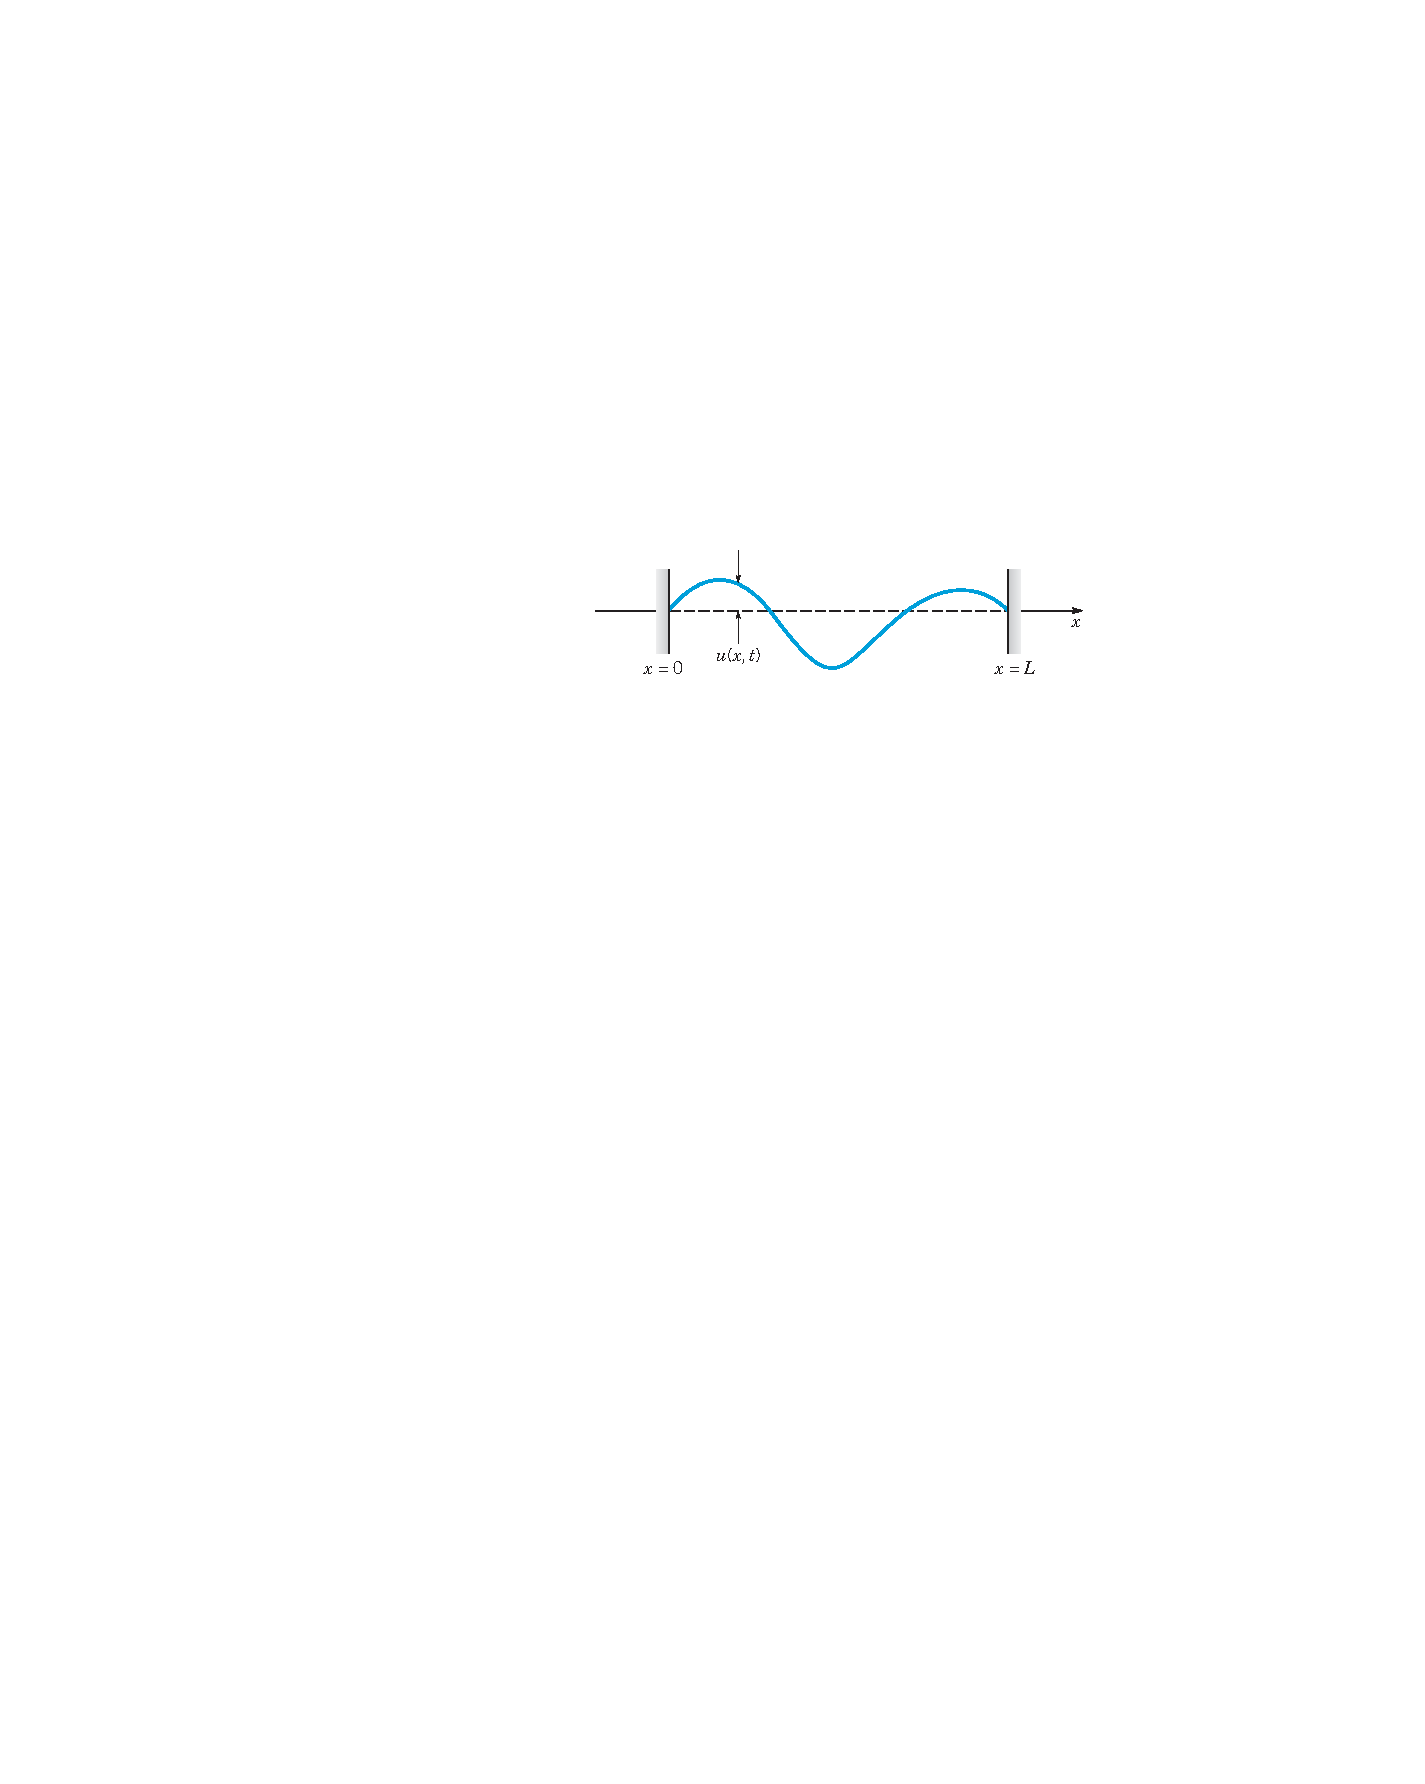
\includegraphics[width=0.7\textwidth]{WaveString.pdf}
	\caption{A vibrating string \cite[Figure 10.7.1]{boyce}.}
	\label{fig:wavestring}
\end{figure}

As before, we use separation of variables, writing
\begin{align*}
	u(x,t) &= X(x) T(t) \\
	\implies XT'' &= a^2 X''T \\
	\implies \frac{1}{a^2} \frac{T''}{T} &= \frac{X''}{X} = \lambda,
\end{align*}
where $\lambda$ is the separation constant.

We first solve the boundary value problem
\[
X'' = \lambda X, \quad X(0) = X(L) = 0.
\]
As was the case when this ODE appeared while solving the heat equation, we find that the eigenvalues are
\[
\lambda_n = -\frac{n^2\pi^2}{L^2},
\]
and the corresponding eigenfunctions are
\[
X_n(x) = \sin\left(\frac{n\pi x}{L}\right), \quad n = 1, 2, \dots.
\]

Now we solve the second ODE:
\[
T_n'' - a^2\lambda T_n = 0 \implies T_n'' + \frac{n^2\pi^2a^2}{L^2}T_n = 0.
\]
Since $\frac{n^2\pi^2a^2}{L^2} > 0$, we have solutions of the usual form:
\[
T_n(t) = a_n \cos\left(\frac{n\pi at}{L}\right) + b_n \sin\left(\frac{n\pi at}{L}\right).
\]

Therefore we have the following elementary solutions
\[
u_n(x,t) = X_n T_n(t) = \left(a_n \cos\left(\frac{n\pi at}{L}\right) + b_n \sin\left(\frac{n\pi at}{L}\right)\right) \sin\left(\frac{n\pi x}{L}\right), 
\]
and a general solution given by
\begin{equation}
	u(x,t) = \sum_{n=1}^{\infty} \left(c_n \cos\left(\frac{n\pi at}{L}\right) + d_n \sin\left(\frac{n\pi at}{L}\right)\right) \sin\left(\frac{n\pi x}{L}\right).
\end{equation}

Now we apply the first of the initial conditions
\[
u(x,0) = \sum_{n=1}^{\infty} c_n \sin\left(\frac{n\pi x}{L}\right) = f(x).
\]
This is nothing but the Fourier series for $f(x)$, with $f(x)$ being an odd function. Therefore, we apply the version of the Euler-Fourier equations found in \Cref{sec:evenoddfourier} to find that
\begin{equation}
	c_n = \frac{2}{L} \int_0^L f(x) \sin\left(\frac{n\pi x}{L}\right).
\end{equation}

Finally, using the second initial condition
\begin{align}
	\p_t u(x,0) &= \sum_{n=1}^{\infty}\frac{n\pi a}{L} d_n \sin\left(\frac{n\pi x}{L}\right) = g(x) \nonumber \\
	\implies \frac{n\pi a}{L} d_n &= \frac{2}{L} \int_0^L g(x) \sin\left(\frac{n\pi x}{L}\right) \nonumber \\
	d_n &= \frac{2}{n\pi a} \int_0^L g(x) \sin\left(\frac{n\pi x}{L}\right).
\end{align}

\begin{eg}\label{eg:waveeqn}
	We consider the case with initial condition $\p_t u = 0$ at $t=0$.
	
	In the case that $u(x,0)$ is given by the tent, we have already calculated the coefficients in \Cref{eg:heateqn1}. Thus the solution is given by, 
	\[
	u(x,t) = \sum_{k=0}^{\infty} \frac{8}{((2k+1)\pi)^2} (-1)^k \sin\left((2k+1)\pi x\right)\cos\left((2k+1)\pi t\right).
	\]
	This solution is shown in \Cref{fig:heateqneg1} for a few select values of $t$.
\end{eg}

\begin{figure}[!ht]
	\centering
	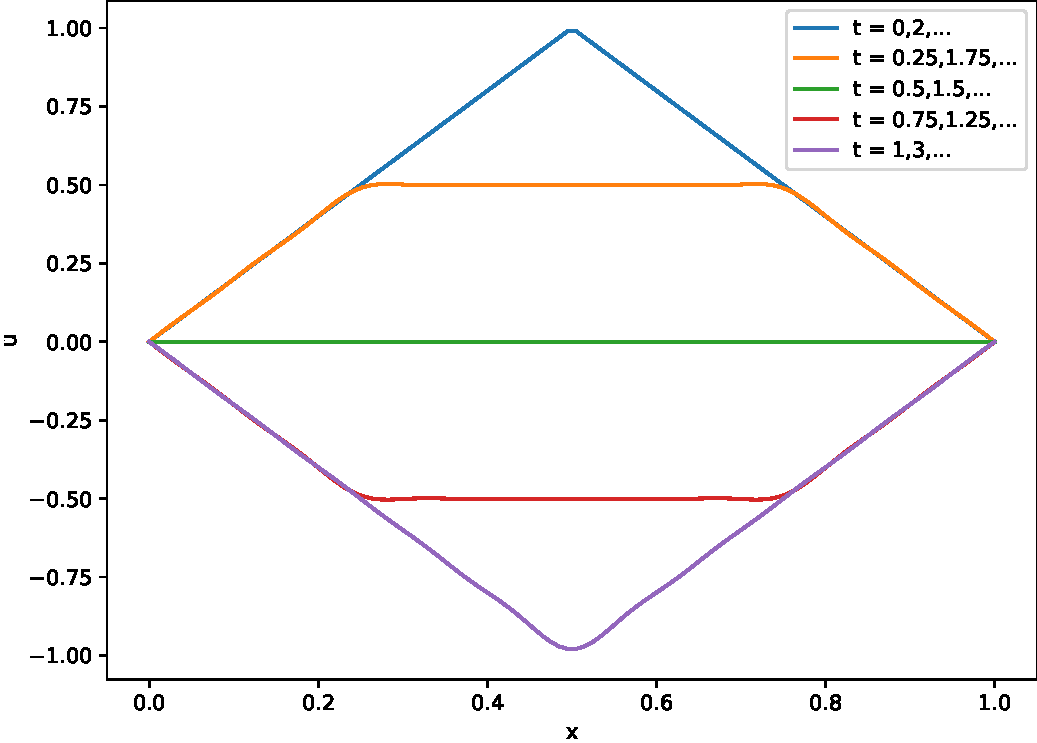
\includegraphics[width=0.7\textwidth]{WaveEqn.pdf}
	\caption{Solution of the heat equation given the initial conditions in \Cref{eg:waveeqn}.}
	\label{fig:waveeqn}
\end{figure}

\begin{eg}
	Let's see how we can interpret the solution of the wave equation when there is no initial velocity ($g(x) = 0$). This means that $d_n = 0$ for all $n$ so the solution is
	\[
	u(x,t) = \sum_{n=1}^{\infty} c_n \cos\left(\frac{n\pi at}{L}\right) \sin\left(\frac{n\pi x}{L}\right).
	\]
	The frequency of the cosine wave will be $f_n = \frac{1}{T_n} = \frac{n\pi a}{2L}$, where $T_n$ is the period of the wave. This suggests that we can decompose the overall solution as the sum of individual waves with period $\frac12$, $1$, $\frac32$, etc. as illustrated in \Cref{fig:harmonics}. These waves are called the fundamental modes of vibration or, in music, they are called the fundamental tone (or first harmonic), second harmonic, and so on.
\end{eg}

\begin{figure}[!ht]
	\centering
	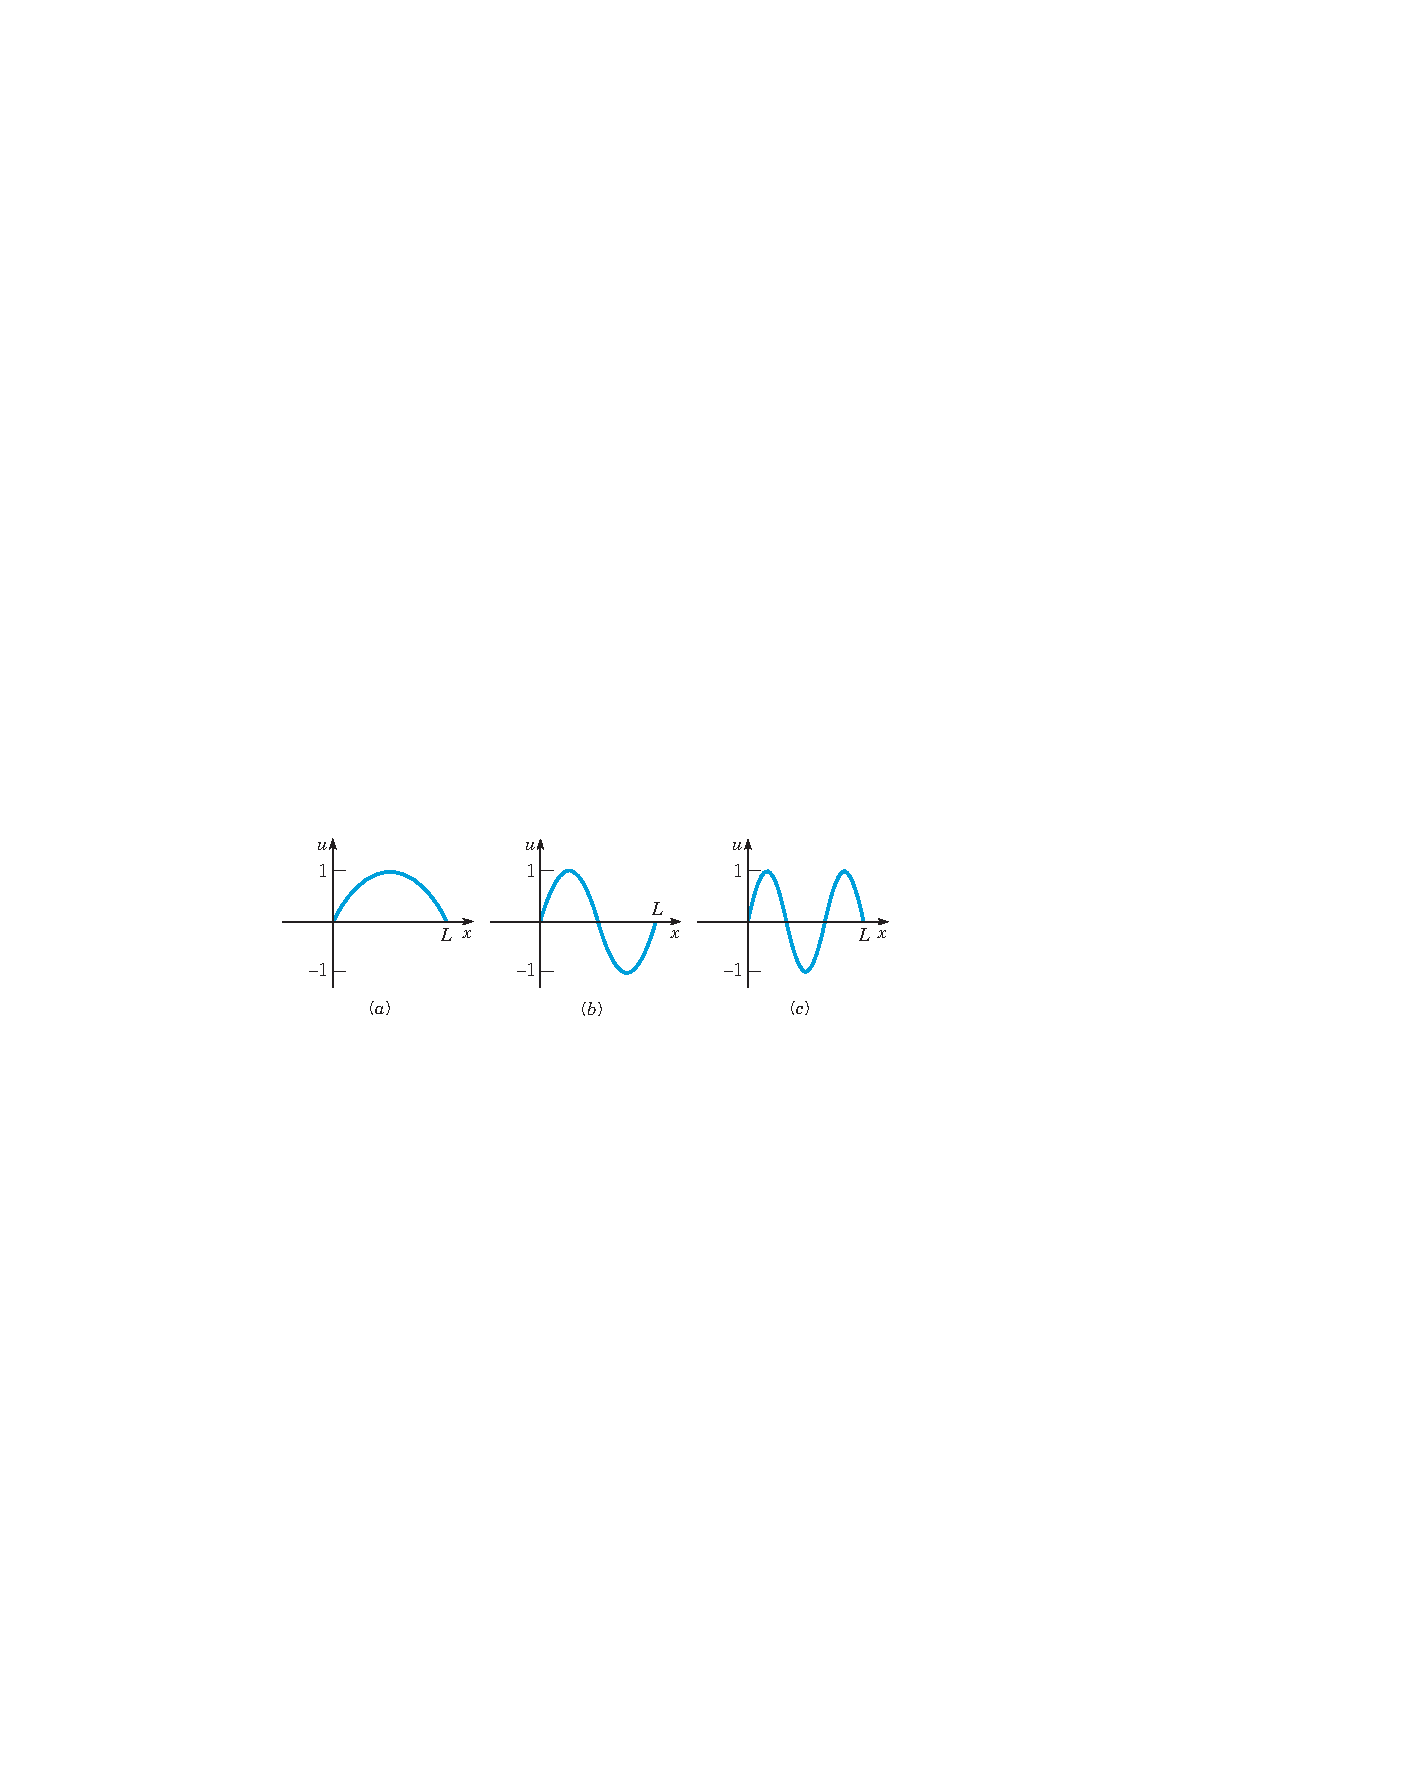
\includegraphics[width=0.7\textwidth]{Harmonics.pdf}
	\caption{First three harmonics for vibration in an elastic string, with frequencies (a) $\frac{\pi a}{L}$, (b) $\frac{2\pi a}{L}$, and (c) $\frac{3\pi a}{L}$ \cite[Figure 10.7.3]{boyce}.} 
	\label{fig:harmonics}
\end{figure}

\subsubsection{D'Alembert's Solution of the Wave Equation}

Considering the one-dimensional wave equation
\[
	\p_{tt} = a^2\p_{xx}u,
\]
let's change coordinates:
\[
	\xi = x - at, \quad \eta = x + at.
\]
Now we rewrite the PDE in new coordinates $u(\xi, \eta)$. To determine the partial derivatives, we need to use the chain rule. First
\[
	\frac{\p u(\xi, \eta)}{\p x} = \p_{\xi}u\frac{\p\xi}{\p x} + \p_{\eta}u\frac{\eta}{\p x} = \p_{\xi}u + \p_{\eta}u.
\]
Iterating the process:
\begin{align*}
	\frac{\p^2u}{\p x^2} &= \frac{\p}{\p x}(\p_{\xi}u + \p_{\eta}u) \\
	&= \p_{\xi\xi}u \p_x\xi + \p_{\eta\xi}u \p_x\eta + \p_{\xi\eta}u \p_x\xi + \p_{\eta\eta}u \p_x\eta \\
	&= \p_{\xi\xi}u + \p_{\eta\eta}u + 2\p_{\xi\eta}u.
\end{align*}
Now using the chain rule again:
\[
	\frac{\p u(\xi, \eta)}{\p t} = \p_{\xi}u\frac{\p\xi}{\p t} + \p_{\eta}u\frac{\eta}{\p t} = -a(\p_{\xi}u - \p_{\eta}u).
\]
And iterating again:
\[
	\frac{\p^2x}{\p t^2} = -a\frac{\p}{\p t} (\p_{\xi}u - \p_{\eta}u) = a^2\p_{\xi\xi}u + a^2\p_{\eta\eta}u - 2a^2\p_{\xi\eta}u.
\]
Bringing this all together:
\begin{align*}
	\p_{tt} &= a^2\p_{xx}u \\
	a^2\p_{\xi\xi}u + a^2\p_{\eta\eta}u - 2a^2\p_{\xi\eta}u &= a^2\p_{\xi\xi}u + a^2\p_{\eta\eta}u + 2a^2\p_{\xi\eta}u \\
	\iff \frac{\p^2u}{\p\xi\p\eta} &= 0 = \frac{\p}{\p\xi}\left(\frac{\p u}{\p\eta}\right).
\end{align*}
So
\[
	\frac{\p u}{\p\eta} = p'(\eta) \implies \frac{\p}{\p\eta}(u - p(\eta)) = 0 \implies u = p(\eta) + q(\xi),
\]
where functions $p$ and $q$ are arbitrary. Therefore, in conclusion
\[
	\p_{tt} = a^2\p_{xx}u \implies u(x,t) = p(x+at) + q(x-at),
\]
which is called D'Alembert's solution.
\begin{itemize}
	\item If $q(x)$ represents a perturbation centred at $x=0$, then $q(x-at)$ describes a perturbation travelling at speed $a$ to the right (i.e. $x>0$ direction).
	\item If $p(x)$ represents a perturbation centred at $x=0$, then $p(x+at)$ describes a perturbation travelling at speed $a$ to the left (i.e. $x>0$ direction).
\end{itemize}


\subsection{Laplace's Equation}

Laplace's equation is given by
\begin{equation}
	\nabla^2u = \p_{xx}u + \p_{yy}u = 0.
\end{equation}

This equation is time-independent and is widely used in physics describing situations of equilibrium, or those that do not depend explicitly on time, such as modelling the shape of soap bubbles or dispersion of heat in a steady state. Since the equation is not dependent on time, there are no initial conditions; only boundary conditions.

There are two different types of boundary conditions to consider:
\begin{itemize}
	\item Dirichlet BCs: function $u(x,y)$ specified at the boundary.
	\item Neumann BCs: normal derivative of $u(x,y)$ specified at the boundary.
\end{itemize}

We will solve Laplace's equation with Dirichlet boundary conditions on two domains: on a rectangle and on a circle.

\begin{enumerate}
	\item \textbf{Laplace's equation on a rectangle.}
	
	We solve
	\[
	\p_{xx}u + \p_{yy}u = 0 \quad \text{in} \quad 0 \leq x \leq a, \,\, 0 \leq y \leq b
	\]
	with the following boundary conditions
	\[
	u(x,0) = u(x,b) = u(0,y) = 0
	\]
	\[
	u(a,y) = f(y).
	\]
	As usual, we use separation of variables:
	\begin{align*}
		u(x,y) &= X(x)Y(y) \\
		\implies 0 &= X''Y + XY''\\
		\implies \frac{X''}{X} &= -\frac{Y''}{Y} = \lambda,
	\end{align*}
	where $\lambda$ is the usual separation constant.
	
	Based on the boundary conditions, it is easier to first solve
	\[
	Y'' = -\lambda Y, \quad Y(0) = Y(b) = 0.
	\]
	This is a boundary value problem we've solved before, with the following eigenvalues and eigenfunctions:\footnote{Note that the coefficient of $Y$ has the opposite sign to the previous examples, so now there is a non-trivial solution only if $\lambda>0$ i.e. $-\lambda<0$.}
	\[
	\lambda_n = \frac{n^2\pi^2}{b^2}, \quad Y_n(y) = \sin\left(\frac{n\pi y}{b}\right).
	\]
	Now we solve the second equation
	\[
	X'' = \lambda X \implies X'' - \frac{n^2\pi^2}{b^2}X = 0, \quad X(0)=0.
	\]
	Same as before, we find that the solutions are of the form
	\[
	X(x) = A\cosh\left(\frac{n\pi x}{b}\right) + B\sinh\left(\frac{n\pi x}{b}\right).
	\]
	Applying the initial condition, we find $X(0) = 0 = A$, therefore the final eigenfunction is given by
	\[
	X_n(x) = \sinh\left(\frac{n\pi x}{b}\right).
	\]
	In sum, we have elementary solutions of the form
	\[
	u_n(x,t) = X_n(x) Y_n(y) = \sinh\left(\frac{n\pi x}{b}\right) \sin\left(\frac{n\pi y}{b}\right),
	\]
	and using superposition to find the general solution yields
	\begin{equation}
		u(x,y) = \sum_{n=1}^{\infty} c_n \sinh\left(\frac{n\pi x}{b}\right) \sin\left(\frac{n\pi y}{b}\right).
	\end{equation}
	All that remains is to use the final boundary condition:
	\[
	u(a,y) = f(y) = \sum_{n=1}^{\infty} c_n \sinh\left(\frac{n\pi a}{b}\right) \sin\left(\frac{n\pi y}{b}\right).
	\]
	This is recognisable as the Fourier series for an odd function or odd extension, where $c_n \sinh\left(\frac{n\pi a}{b}\right)$ are the Fourier coefficients. Therefore applying the Euler-Fourier formulas, we get
	\begin{align}
		c_n \sinh\left(\frac{n\pi a}{b}\right) &= \frac{2}{b} \int_0^b f(y)\sin\left(\frac{n\pi y}{b}\right)dy \nonumber \\
		c_n &= \frac{2}{b\sinh\left(\frac{n\pi a}{b}\right)} \int_0^b f(y)\sin\left(\frac{n\pi y}{b}\right)dy.
	\end{align}
	
	\begin{eg}\label{eg:laplacerect}
		We solve Laplace's equation on the rectangle $0 \leq x \leq 1$, $0 \leq y \leq 1$, where the boundary condition has $f(y)$ being the tent function
		\[
		f(y) = \begin{cases} 2y & \text{if } y \leq \frac12 \\ 2(1-y) & \text{if } y>\frac12 \end{cases}.
		\]
		In order to calculate $c_n$, we need to evaluate
		\begin{align*}
			\int_0^b f(y)\sin\left(\frac{n\pi y}{b}\right)dy &= \int_0^1 f(y)\sin(n\pi y) \,dy \\
			&= \int_0^{1/2} 2y\sin(n\pi y) \,dy + \int_{1/2}^1 2(1-y)\sin(n\pi y) \,dy.
		\end{align*}
		Evaluating the first integral
		\begin{align*}
			\int_0^{1/2} 2y\sin(n\pi y) \,dy &= \left[ -\frac{2}{n\pi}y\cos(n\pi y)\right]_0^{1/2} + \int_0^{1/2} \frac{2}{n\pi} \cos(n\pi y) \,dy \\
			&= \frac{2}{n\pi}\left[-y\cos(n\pi y)\right]_0^{1/2} + \frac{2}{n^2\pi^2}\left[\sin(n\pi y)\right]_0^{1/2} \\
			&= -\frac{1}{n\pi} \cos\left(\frac{n\pi}{2}\right) + \frac{2}{n^2\pi^2} \sin\left(\frac{n\pi}{2}\right).
		\end{align*}
		And now turning to the second integral
		\begin{align*}
			&\int_{1/2}^1 2(1-y)\sin(n\pi y) \,dy \\
			&= \int_{1/2}^1 2\sin(n\pi y) \,dy - \int_{1/2}^1 2y\sin(n\pi y) \,dy \\
			&= 2\left(\left[-\frac{1}{n\pi}\cos(n\pi y)\right]_{1/2}^1 - \left( \left[-\frac{1}{n\pi}y\cos(n\pi y)\right]_{1/2}^1 + \int_{1/2}^1 \frac{1}{n\pi}\cos(n\pi y) \,dy \right)\right) \\
			&= 2\left(\frac{\cos(n\pi/2)}{n\pi} -\cancel{\frac{\cos(n\pi)}{n\pi}} + \cancel{\frac{\cos(n\pi)}{n\pi}} - \frac{\cos(n\pi/2)}{2n\pi} + \cancelto{0}{\frac{\sin(n\pi)}{n^2\pi^2}} + \frac{\sin(n\pi/2)}{n^2\pi^2}\right) \\
			&= \frac{1}{n\pi} \cos\left(\frac{n\pi}{2}\right) + \frac{2}{n^2\pi^2} \sin\left(\frac{n\pi}{2}\right).
		\end{align*}
		Summing these two expressions, the original integral is
		\begin{align*}
			\int_0^1 f(y)\sin(n\pi y) \,dy &= \frac{4}{n^2\pi^2} \sin\left(\frac{n\pi}{2}\right) \\
			\implies c_n &= \frac{8}{n^2\pi^2\sinh(n\pi)} \sin\left(\frac{n\pi}{2}\right)
		\end{align*}
		We know $\sin(n\pi/2)$ is non-zero only for odd $n$, oscillating between 1 and -1. Therefore, the final solution can be written as 
		\[
		u(x,y) = 8\sum_{n=0}^{\infty} \frac{(-1)^n}{(2n+1)^2\pi^2 \sinh\left((2n+1)\pi\right)} \sinh\left((2n+1)\pi x\right) \sin\left((2n+1)\pi y\right),
		\] 
		which is shown in \Cref{fig:laplacerect}
	\end{eg}
	
	\begin{figure}[!ht]
		\centering
		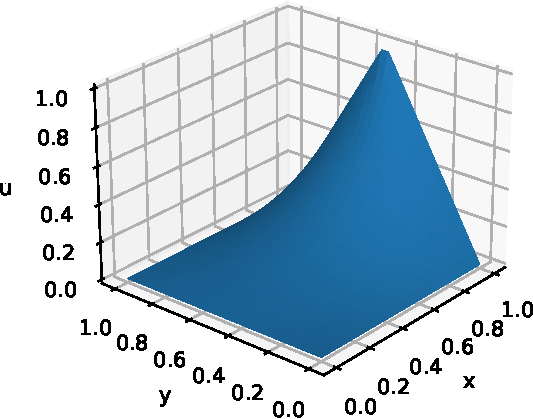
\includegraphics[width=0.7\textwidth]{LaplaceRect.pdf}
		\caption{The solution of Laplace's equation with the boundary conditions $u(x,0) = u(x,b) = u(0,y) = 0$ and $u(a,y) = f(y)$, where $f(y)$ is the tent function. Intuitively, this may be thought of as the shape a soap bubble would take given these boundary conditions.}
		\label{fig:laplacerect}
	\end{figure}
	
	\item \textbf{Laplace's equation on a disc.}
	
	In this case, we solve
	\[
		u_{xx} + u_{yy} = 0
	\]
	with boundary equations expressed in polar coordinates,
	\[
		u(r=a, \theta) = f(\theta), \quad u(r,\theta) \text{ bounded for } r \leq a.
	\]
	To proceed, we need to change Laplace's equation into polar coordinates, which is\footnote{For a derivation of this, see \url{https://www.math.ucdavis.edu/~saito/courses/21C.w11/polar-lap.pdf}.}
	\begin{align*}
		\frac{1}{r}(r u_r)_r + \frac{1}{r^2}u_{\theta\theta} &= 0 \\
		\frac{\p^2u}{\p r^2} + \frac{1}{r}\frac{\p u}{\p r} + \frac{1}{r^2}\frac{\p^2u}{\p\theta^2} &= 0.
	\end{align*}
	
	Now to solve this equation, we use the usual method of separation of variables
	\begin{align*}
		u(r, \theta) &= R(r)\Theta(\theta) \\
		0 &= \frac{1}{r}(r R_r)_r\Theta + \frac{1}{r^2}R \Theta_{\theta\theta} \\
		\frac{r(rR')'}{R} &= -\frac{\Theta''}{\Theta} = \lambda,
	\end{align*}
	where in the final line we use $R'$ and $\Theta'$ to denote differentiation with respect to the relevant independent variable since $R$ and $\Theta$ are functions of one variable.
	
	Now, we shall solve $\Theta'' = -\lambda\Theta$, using the condition that $\Theta$ must be $2\pi$-periodic in $\theta$. As usual, we have three cases:
	\begin{itemize}
		\item Case 1: $\lambda = \mu^2 > 0$. Then the solution is
		\[
		\Theta = A\cos(\mu\theta) + B\sin(\mu\theta),
		\]
		where $\mu = n = 1, 2, \dots$ for $2\pi$-periodic solutions.
		\item Case 2: $\lambda=0$. The solution is
		\[
		\Theta = A\theta + B,
		\]
		which implies that $\Theta$ is constant for it to be periodic.
		\item Case 3: $\lambda = -\mu^2 < 0$. The solution is
		\[
		\Theta = A\cosh(\mu\theta) + B\sinh(\mu\theta),
		\]
		which is never periodic, thus there are no solutions.
	\end{itemize}
	
	So overall, the eigenvalues are
	\[
	\lambda_0 = 0 \quad \text{and} \quad \lambda_n = n^2,
	\]
	and the corresponding eigenfunctions are
	\[
	\Theta_0(\theta) = 1 \quad \text{and} \quad \Theta_n(\theta) = c_n\cos(n\theta) + d_n\sin(n\theta).
	\]
	Alternatively, we may split the eigenfunction $\Theta_n$ into two separate functions:
	\[
	\Theta_n(\theta) = \cos(n\theta) \quad \text{and} \quad \widetilde{\Theta}_n(\theta) = \sin(n\theta).
	\]
	
	Now, we turn to solving the second equation, $\frac{r(rR')'}{R} = \lambda \iff r(rR')' = n^2R$. We split this into two cases:
	\begin{itemize}
		\item Case 1: $n=0$. In this case, the equation becomes
		\[
		(rR')' = 0 \implies rR' = A \implies R = \cancelto{0}{A\log r} + B
		\]
		since the solution must be bounded (so we cannot have $\log r$ being unbounded as $r \to 0$). Therefore the solution in this case is constant.
		\item Case 2: $n = 1, 2, \dots$. The equation becomes
		\[
		r^2R'' + rR' - n^2R = 0,
		\]
		which is an Euler equation. To solve such equations, we try $R(r) = r^{\alpha}$, yielding
		\begin{align*}
			\alpha(\alpha-1)r^{\alpha} + \alpha r^{\alpha} - n^2r^{\alpha} &= 0 \\
			\alpha^2 &= n^2 \\
			\alpha &= \pm n.
		\end{align*}
		Therefore
		\[
		R(r) = Ar^n + \cancelto{0}{Br^{-n}},
		\]
		where we cancel $r^{-n}$ by setting $B=0$ so that the solution is bounded as $r\to 0$.
	\end{itemize}
	Putting all this together, we have the following elementary solutions
	\[
	u_0(r,\theta) = 1, \quad u_n(r,\theta) = r^n\cos(n\theta), \quad \widetilde{u}_n(r,\theta) = r^n\sin(n\theta),
	\]
	and using superposition to find the general solution yields
	\begin{equation}\label{eq:laprectgensol}
		u(r,\theta) = a_0 + \sum_{n=1}^{\infty} r^n\left(a_n\cos(n\theta) + b_n\sin(n\theta)\right).
	\end{equation}
	
	To complete the solution, we use the given boundary condition 
	\[
	u(a, \theta) = \frac{a_0}{2} + \sum_{n=1}^{\infty} a_na^n \cos(n\theta) + b_na^n \sin(n\theta) = f(\theta).
	\]
	This is nothing but a Fourier series with $2L = 2\pi$ and Fourier coefficients $a_na^n$ and $b_na^n$.\footnote{Observe that we have replaced $a_0$ with $\frac{a_0}{2}$ to match the Fourier series form.} By the usual method of using the Euler-Fourier equations, we find that
	\begin{align}
		\label{eq:lapdisccoeff1}
		a_n &= \frac{1}{a^n\pi} \int_{-\pi}^{\pi} f(\theta) \cos(n\theta) \,d\theta \\
		\label{eq:lapdisccoeff2}
		b_n &= \frac{1}{a^n\pi} \int_{-\pi}^{\pi} f(\theta) \sin(n\theta) \,d\theta \\
		a_0 &= \frac{1}{\pi} \int_{-\pi}^{\pi} f(\theta) \,d\theta
	\end{align}
	
	\begin{remark}
		If $f(\theta)$ is an odd function, then the integrand $f(\theta) \cos(n\theta)$ in \Cref{eq:lapdisccoeff1} is odd, so $a_n=0$ and the terms in $\cos(n\theta)$ vanish. Similarly, if $f(\theta)$ is an even function, $f(\theta) \sin(n\theta)$ in \Cref{eq:lapdisccoeff2} is odd and $b_n=0$ for all $n$.
	\end{remark}
	
	\begin{remark}
		The more general solution for Laplace's equation on the annulus $r_1 \leq r \leq r_2$, $-\pi \leq \theta \leq \pi$ is
		\begin{equation}
			u(r,\theta) = \frac{a_0}{2} + \frac{\hat{a}_0}{2}\log{r} + \sum_{n=1}^{\infty} \left(a_nr^n + \hat{a}_nr^{-n}\right)\cos(n\theta) + \sum_{n=1}^{\infty} \left(b_nr^n + \hat{b}_nr^{-n}\right)\sin(n\theta)
		\end{equation}
		for arbitrary real constants $a_n$, $\hat{a}_n$, $b_n$, and $\hat{b}_n$. Note that this becomes the solution in \Cref{eq:laprectgensol} when we take $r_1=0$ and impose $\hat{a}_n = \hat{b}_n = 0$ for all $n$ so the solution is bounded.
	\end{remark}
	
	\begin{eg}
		We solve Laplace's equation on the disc $r \leq 1$ with the boundary conditions
		\[
		u(1, \theta) = \begin{cases} 1 & \text{if } -\frac{\pi}{2} < \theta < \frac{\pi}{2} \\ 0 & \text{otherwise} \end{cases}.
		\]
		Solving for $a_n$ and $b_n$ is much easier than in \Cref{eg:laplacerect}, therefore this working is left as an exercise. We note only that solution is 
		\[
		u(r,\theta) = \sum_{n=1}^{\infty} \frac{2}{n\pi}\sin\left(\frac{n\pi}{2}\right) r^n \cos(n\theta),
		\] 
		which is shown in \Cref{fig:laplacecircle}.
	\end{eg}
	
	\begin{figure}[!ht]
		\centering
		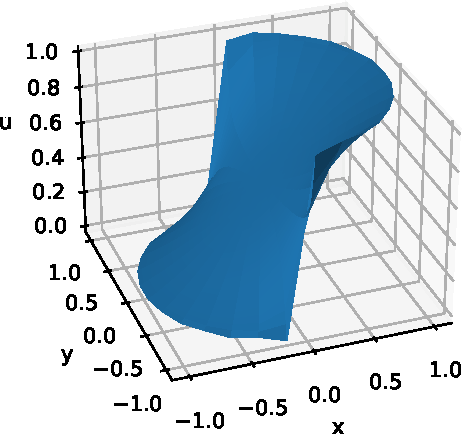
\includegraphics[width=0.7\textwidth]{LaplaceCircle.pdf}
		\caption{The solution of Laplace's equation on a disc.}
		\label{fig:laplacecircle}
	\end{figure}
\end{enumerate}

\pagebreak
\subsection{Summary}

Given a linear PDE for $u(x,t)$:
\begin{itemize}
	\item Assume separation of variables: $u(x,t) = X(x)T(t)$.
	\item Introduce a separation of variables constant $\lambda$.
	\item Identify the eigenvalue boundary problem satisfied by $X(x)$ and $\lambda$, which depends upon the boundary conditions.
	\item Solve for $X(x)$: this step may require some quantisation of $\lambda$ or some constraint on $\lambda$.
	\item Solve the eigenvalue initial problem satisfied by $T(t)$.
	\item Write the most general solution as a linear combination of all solutions to the eigenvalue boundary/initial problems.
	\item Identify any undetermined coefficients using initial conditions.
	\item Note that there can be more than one separation constant if number of independent variables is greater than 2, e.g. $u(x,y,t)$.
We will see this later in \Cref{sec:waveeqn2d} when we study the wave equation in two dimensions.
\end{itemize}